\section{Autres systèmes}
\subsection{Précision}
Il existe de nombreux systèmes d'exploitation qui nous sont, en partie,
inconnus. \\

La raison est simple: les systèmes d'exploitation que nous connaissons ont dû se
développer sur base de systèmes d'exploitation expérimentaux qui ne sont plus
utilisés. \\

Exemple : \\

\begin{itemize}
\item Singularity : utilisé pour les recherches de Microsoft; \\

\item MyOS : mini système d'exploitation créé à l'aide du langage C++; \\

\item Desert Spring-Time (\textit{DST}) : système d'exploitation développé en
Objective Caml; \\

\item Kid Operating System (\textit{KOS}) : utilisé pour l'apprentissage; \\

\item (\textbf{...}) \\
\end{itemize}

En outre, il y a des systèmes d'exploitation pour smartphone qui ont été mis de
côté suite à l'abandon de leur développement au profit d'autres technologies. \\

Exemple : \\

\begin{itemize}
\item Symbian : développé par Nokia; \\

\item Meego : développé par Nokia et Intel; \\

\item BlackberryOS : développé par Research In Motion; \\

\item Bada : développé par Samsung; \\

\item (\textbf{...})
\end{itemize}

\newpage

De plus, la majorité des appareils électriques ont un système d'exploitation,
nommé \textit{système embarqué}. \\
C'est lui qui permet de gérer l'aspect informatique du composant; de même, que
d'offrir une interface graphique conviviale à l'utilisateur pour interagir avec
ces appareils. \\

Par exemple, il en existe pour la télévision: \\

\begin{itemize}
\item Tizen : développé par Samsung; \\

\item WebOS : développé par LG; \\

\item tvOS : développé par Apple pour l'Apple TV; \\

\item Android TV : développé par Android; \\

\item (\textbf{...}) \\
\end{itemize}

Les voitures et les camions possèdent un ordinateur intégré qui les contrôle,
comme l'ABS (\textit{système antiblocage des roues}) qui est contrôlé par
l'ordinateur de bord. \\
L'un des plus gros problèmes est la sécurité. \\En effet, si un malandrin pirate
le système d'une voiture, il peut très bien couper le moteur de la voiture au
beau milieu de l'autoroute et le conducteur ne pourra même pas le rallumer ! \\
Ce qu'il faudrait alors, c'est mettre à jour le système, un peu comme pour les
\textit{Teslas} qui reçoivent des mises à jour par Internet, mais le procédé
n'est pas encore assez fiable…

\clearpage

\subsection{Cisco IOS}
Cisco IOS (\textit{Internetwork Operating System}) est le leader mondial des
systèmes d'exploitation de réseau, il est développé par \textit{Cisco Systems}
et équipe la plupart de leurs équipements.

\begin{figure}[!h]
  \centering
  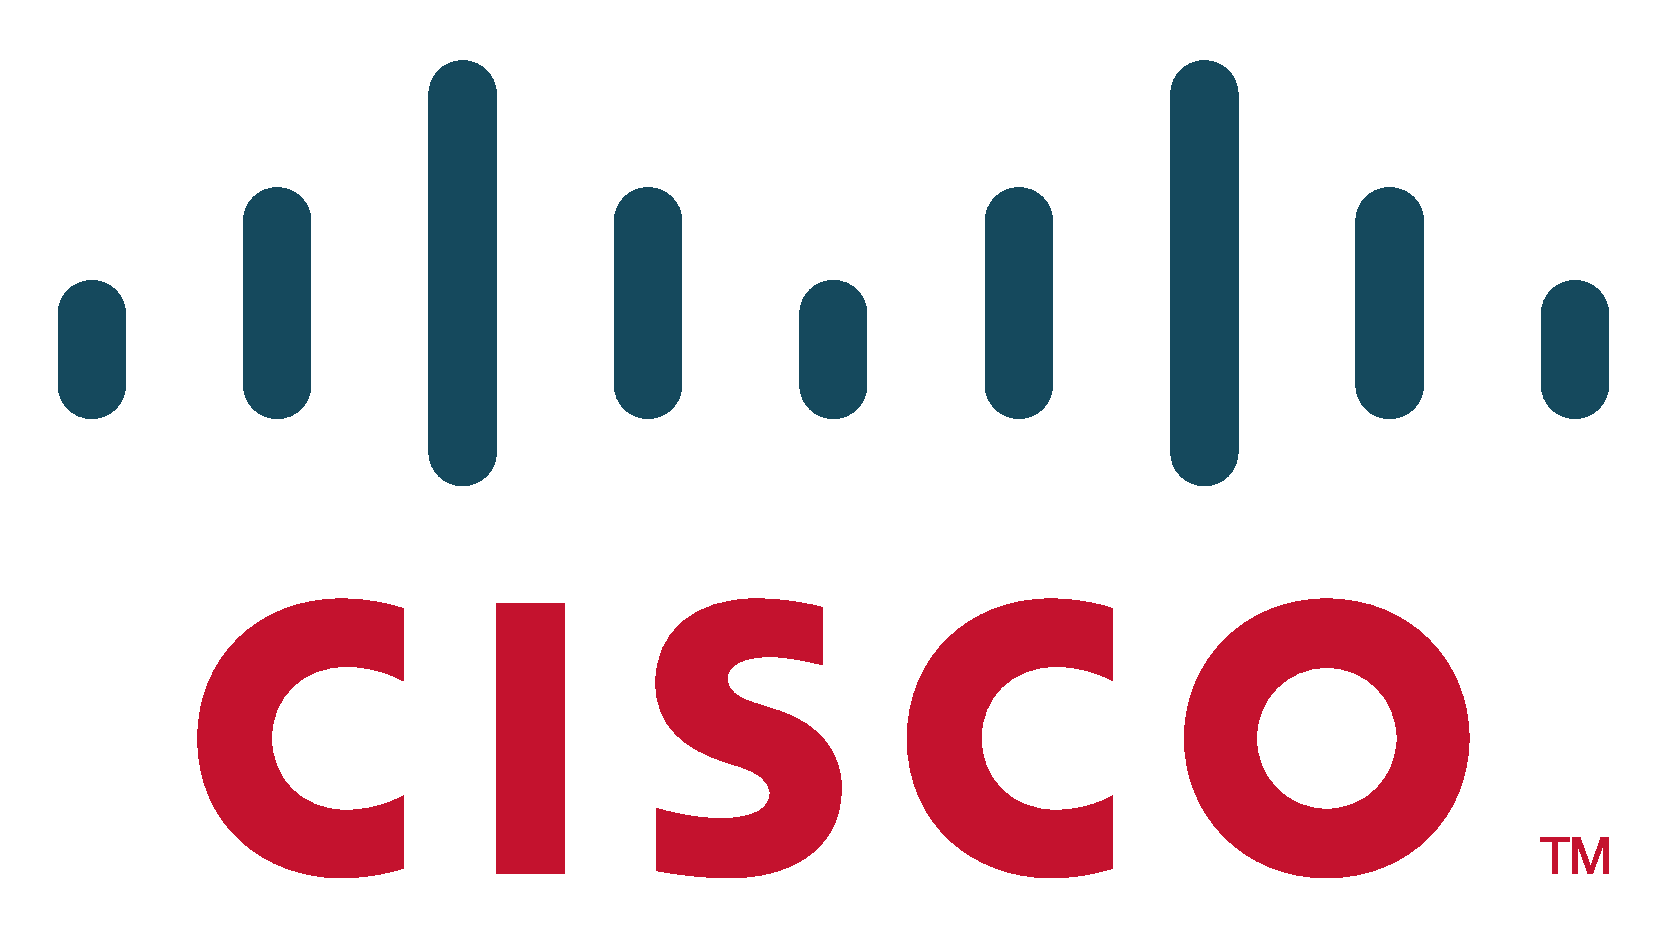
\includegraphics[scale=0.15]
  {textures/images/others/Cisco_logo.pdf}
  \caption{Logo de Cisco Systems}
\end{figure}

Il est décliné en différentes versions spécialisées pour chaque équipement
(\textit{routeur, commutateur, points d’accès Wi-Fi,…}). \\
L’accès se fait par le port console (ou auxiliaire), Telnet ou SSH, et en ligne
de commande (\textbf{CLI}) ou par une interface web. \\

Du côté de la sécurité, l’accès au périphérique et l’accès au mode d’exécution
privilégié peuvent être protégés par un mot de passe de même. \\

En effet, il existe plusieurs modes d’exécution:

\begin{enumerate}
\item le mode d’exécution utilisateur : point d’entrée de base de la CLI,
  les commandes y sont restreintes;

\item le mode d’exécution privilégié : il permet d’accéder aux informations
  détaillées et aux commandes de configuration et de gestion du périphérique;

\item le mode de configuration globale : permet d’effectuer des commandes de
  configuration globales sur l’équipement;

\item les autres sous-modes : accessibles depuis le mode global, ils permettent
  de configurer des interfaces (\textit{Vlan, VTY, etc.}). \\
\end{enumerate}

Il existe d’autres systèmes d’exploitation de Cisco. \\
Par exemple:

\begin{itemize}
\item CatOS : répandu dans les commutateurs Ethernet haut de gamme, il provient
  de la gamme de commutateurs Catalyst;

\item IOS XE : basé sur Linux, il est compatible avec IOS et est utilisé par les
  entreprises et les fournisseurs de services;

\item NX-OS : pour les commutateurs Ethernet Nexus et les commutateurs à fibre
  optique MDS. Il est basé sur SAN-OS, développé à l'origine pour les commutateurs
  MDS.
\end{itemize}
